\section{Further Studies}

The obtained results using the QR methodology give incentives to keep doing experiments and finding new aspects which could help improve the process of generating scenarios. Of the many possible paths, the following are the next steps to be investigated by the researchers. 

\subsection{Information Criteria for Quantile Regression}
Using CV can be computationally expensive, as the full estimation is done several times for each tuning parameter - in this case, $\gamma$ and $\lambda$. Other form of deciding the quantity of variables that provides a good equilibrium between in-sample prediction and parsimony is the Information Criteria.

Information criteria summarizes two aspects. One of them refers to how well the model fits the in-sample observations and the other part penalizes the quantity of covariates used in the model. By penalizing how big our model is, we prevent overfitting from happening. So, in order for a covariate to be included in the model, it must supply enough goodness of fit.
In \cite{machado1993robust}, it is presented a variation of the Schwarz criteria for M-estimators that includes quantile regression. The Schwarz Information Criteria (SIC), adapted to the quantile autoregression case, is presented below:
\begin{align} 
\begin{split}
SIC(m) = \sum_{j \in J} \log \left(\sum_{t \in T}\rho_{\alpha_j}(y_t - \beta_0 - \beta^T x_t) \right) +  \frac{\log|T|}{2|T||P|} K(m),\label{eq:SIC}
\end{split}					
\end{align}
where $K(m)$ is the quantity of coefficients $\beta_{pj}$ greater than zero in the model $m$.
By minimizing the $SIC$ function, the chosen model is the one with the best combination, according to this metric, of fit and parsimony among all models. 

Even though CV is very popular and produce great results, selecting model with Information Criteria is much quicker. For the case where the selected model is very similar, it might be the case that the estimation methodology may change a little bit. It is definitely a topic that worths researching.

\subsection{Quantile Autoregression with a nonparametric approach}
\label{sec:npqar}

Fitting a linear estimator for the Quantile Auto Regression is less efficient if nonlinearity is present in the quantile functions. This nonlinearity may produce a linear estimator that underestimates the quantile for a chunk of data while overestimating for the other chunk. To prevent this issue from occurring we propose to use a nonparametric quantile regression model. 
% To sprevent overfitting and smoothen our predictor, we include a penalty on its roughness by including the $\ell_1$ norm of its second derivative. For more information on the $\ell_1$ norm acting as a filter, one can refer to \cite{kim2009ell_1}.

% This time, as opposed to when employing linear models, we don't suppose any functional form for $q_\alpha(x_t)$. This forces us to build each $q_\alpha$ differently: instead of finding a set of parameters that fully defines the function, we find a value for $q_\alpha(x_t)$ at each instant $t$. On the optimization problem, we will find optimal values for a variable $q_{tj} \in \mathbb{R}$, each consisting of a single point. The sequence  $\{ q^*_{\alpha t} \}_{\alpha \in A} $ will provide a discretization for the quantile function $\hat{q}_\alpha(x_t)$, which can be found by interpolating these points.

% notação estatística de ordem. com x^(0)

Let $\{\tilde{y}_t \}_{t=1}^n$ be the sequence of observations in time $t$ and let $\tilde{x}_t$ be the $p-$lagged time series of $\tilde{y}_t$, such that $\tilde{x}_t = L^p(\tilde{y}_t)$, where $L$ is the lag operator. Matching each observation $\tilde{y}_t$ with its $p-$lagged correspondent $\tilde{x}_t$ produces $n-p$ pairs $\{(\tilde{y}_t,\tilde{x}_t)\}_{t=p+1}^n$ (note that the first $p$ observations of $y_t$ must be discarded). When the sequence of observations of $x$ are reorder in such a way that they are in growing order
$$\tilde{x}^{(p+1)} \leq \tilde{x}^{(p+2)} \leq \dots \leq \tilde{x}^{(n)},$$ 
the new sequences can be defined $\{x_i\}_{i=1}^{n-p} = \{\tilde{x}^{(t)} \}_{t=p+1}^{n}$ and $\{y_i\}_{i=1}^{n-p} = \{\tilde{y}^{(t)} \}_{t=p+1}^{n}$, where $T' = \{2,\dots, n-p-1\}$. 

The optimization model to estimate the nonparametric quantile is as follows:
\begin{equation}
\begin{split}
\hat{q}_{\alpha_j}(x_t) =\underset{q_{tj}}{\arg\min}\sum_{t\in T'} \rho_{\alpha_j} \left( y - q_{tj} \right) \\ +\lambda_1  \sum_{t\in T'}|D_{x_t}^{1}q_{tj}| +\lambda_2  \sum_{t\in T'}|D_{x_t}^{2}q_{tj}|,
\end{split}
\end{equation}
where $D^1 q_t$ and $D^2 q_t$ are the first and second derivatives of the $q_\alpha(x_t)$ function, calculated as follows:
\begin{equation*}
D_{x_{t}}^{2}q_{tj}=\frac{\left(\frac{q_{\alpha t+1}-q_{tj}}{x_{t+1}-x_{t}}\right)-\left(\frac{q_{tj}-q_{\alpha t-1}}{x_{t}-x_{t-1}}\right)}{x_{t+1}- x_{t-1}},
\end{equation*}

\begin{equation*}
D^{1}_{tj}=\frac{q_{\alpha t+1}-q_{tj}}{x_{t+1}-x_{t}}.
\end{equation*}
%The first part on the objective function is the usual quantile regression condition for $\{q_{t\alpha}\}_{\alpha \in A}$. The second part is the $\ell_1$-filter. The purpose of a filter is to control the amount of variation for our estimator $q_\alpha(x_t)$. When no penalty is employed we would always get $q_{tj} = y_t$, for any given $\alpha$. On the other hand, when $\lambda_2 \rightarrow \infty$, our estimator approaches the linear quantile regression. 

The full model can be rewritten as a LP problem as bellow:
\begin{IEEEeqnarray}{lcr}
\min_{q_{tj},\varepsilon^+_{tj}, \varepsilon_{tj}^-, \xi_t} & \sum_{j \in J} \sum_{t \in T'}\left({\alpha_j}\varepsilon_{tj}^{+}+(1-{\alpha_j})\varepsilon_{tj}^{-}\right) & \\
& \qquad \qquad \qquad \qquad \qquad + \lambda_1\sum_{t \in T'}\gamma_{tj} + \lambda_2\sum_{t \in T'}\xi_{tj} & \nonumber \\
s.t. & \varepsilon_{t}^{+}-\varepsilon_{tj}^{-}=y_{t}-q_{tj}, & \qquad\forall t \in T',\forall j \in J,\\
   & D^{1}_{tj}=\frac{q_{\alpha t+1}-q_{tj}}{x_{t+1}-x_{t}},
    & \qquad\forall t \in T',\forall j \in J,\\   
 & D^{2}_{tj}=\frac{\left(\frac{q_{\alpha t+1}-q_{tj}}{x_{t+1}-x_{t}}\right)-\left(\frac{q_{tj}-q_{\alpha t-1}}{x_{t}-x_{t-1}}\right)}{x_{t+1}- x_{t-1}}.
  & \qquad\forall t \in T',\forall j \in J,\\
 & \gamma_{t \alpha}\geq D^1_{tj}, & \qquad\forall t \in T',\forall j \in J,\\
  & \gamma_{t \alpha}\geq-D^1_{t \alpha}, & \qquad\forall t \in T',\forall j \in J,\\
  & \xi_{t \alpha}\geq D^2_{tj}, & \qquad\forall t \in T',\forall j \in J,\\
 & \xi_{t \alpha}\geq-D^2_{t \alpha}, & \qquad\forall t \in T',\forall j \in J,\\
 & \varepsilon_{t \alpha}^{+},\varepsilon_{t \alpha}^{-},\gamma_{t \alpha}, \xi_{t \alpha}\geq0, & \qquad\forall t \in T',\forall j \in J,\\
  & q_{t j} \leq q_{t j+1}, & \qquad \forall t \in T', \forall j \in J_{(-1)}
  \end{IEEEeqnarray}


The output of this optimization problem is a sequence of ordered points $\{(x_t, q_{tj})\}_{t \in T}$, for all $j \in J$. The next step is to interpolate these points in order to provide an estimation for any other value of $x_t$. To address this issue, we propose using a linear interpolation. Note that $q_{tj}$ is a variable that represents only one point of the $\alpha_j$-quantile function $q_\alpha(x_t)$. 

The quantile estimation is done for different values of $\lambda_2$. By using different levels of penalization on the second difference, the estimation can be more or less adaptive to the fluctuation. It is important to notice that the usage of the $\ell_1$-norm as penalty leads to a piecewise linear solution $q_{tj}$. % Referenciar?
Figure \ref{fig:npqar-results} shows the quantile estimation for a few different values of $\lambda_2$. 

	
% Para os gráficos antigos, usar a pasta /npqar/
\begin{figure*}[htp]
  \centering
  \begin{minipage}[t]{0.4\linewidth}
    \centering
    \begin{minipage}[t]{\linewidth}
      \centering     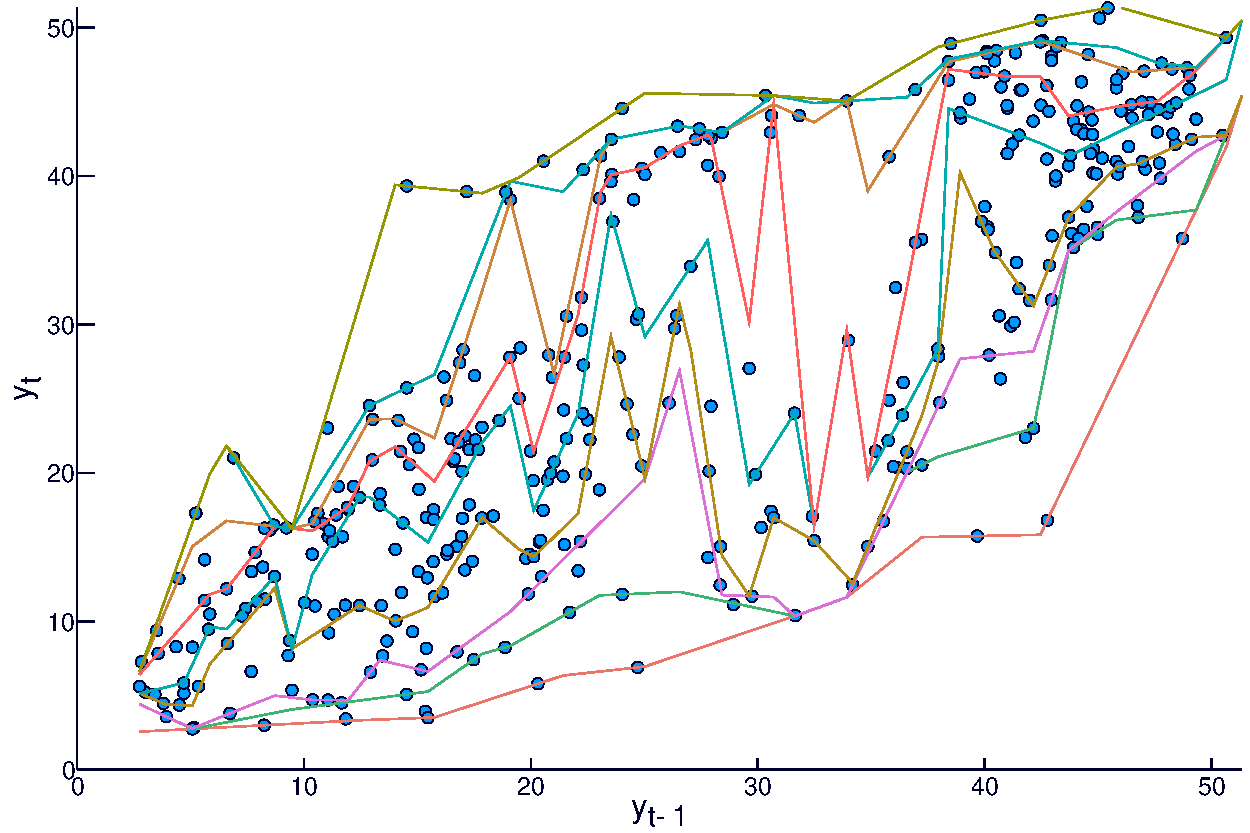
\includegraphics[width=\textwidth]{Figuras-DocRQ/icaraizinho-crossing-01}
      \subcaption{$\lambda_1 = 0, \, \lambda_2 = 0.1$}
    \end{minipage}
    \begin{minipage}[b]{\linewidth}
      \centering     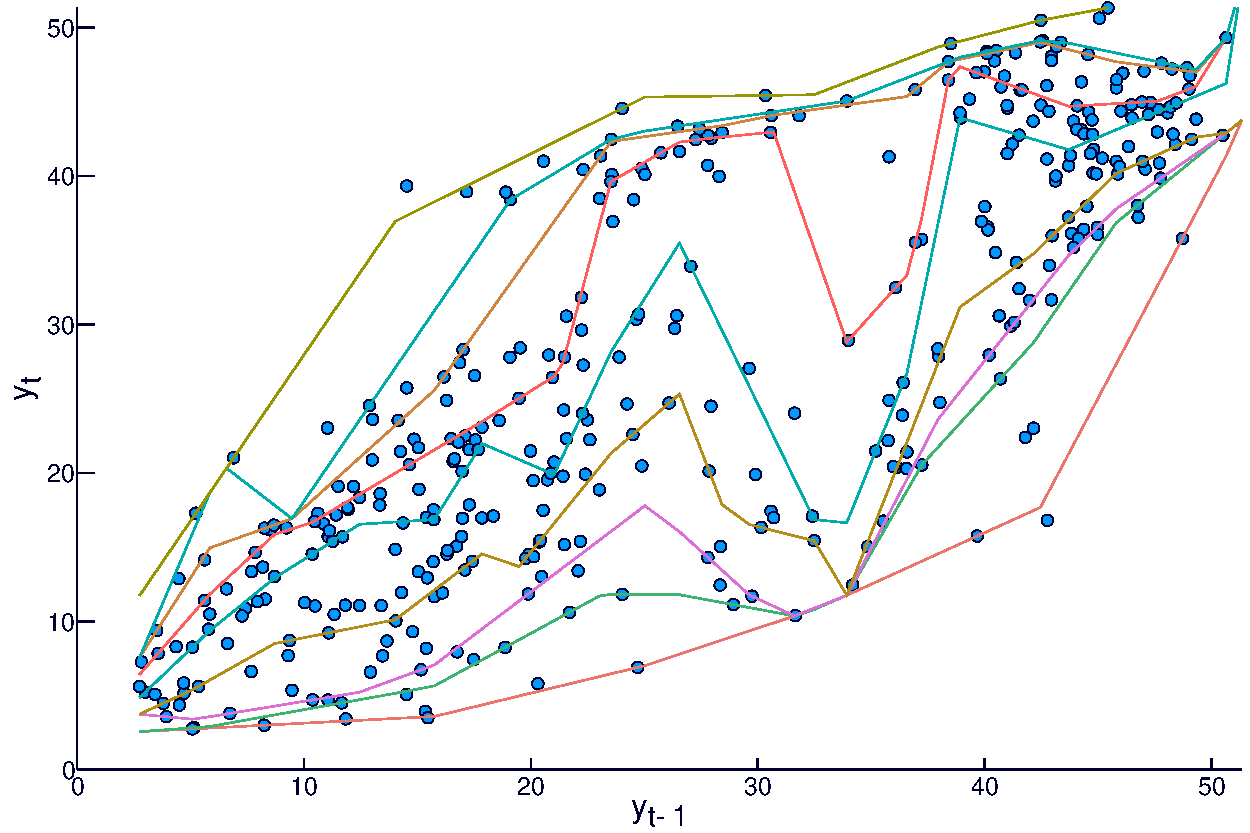
\includegraphics[width=\textwidth]{Figuras-DocRQ/icaraizinho-crossing-03}
      \subcaption{$\lambda_1 = 0, \, \lambda_2 = 0.3$}
    \end{minipage}
     \begin{minipage}[b]{\linewidth}
      \centering     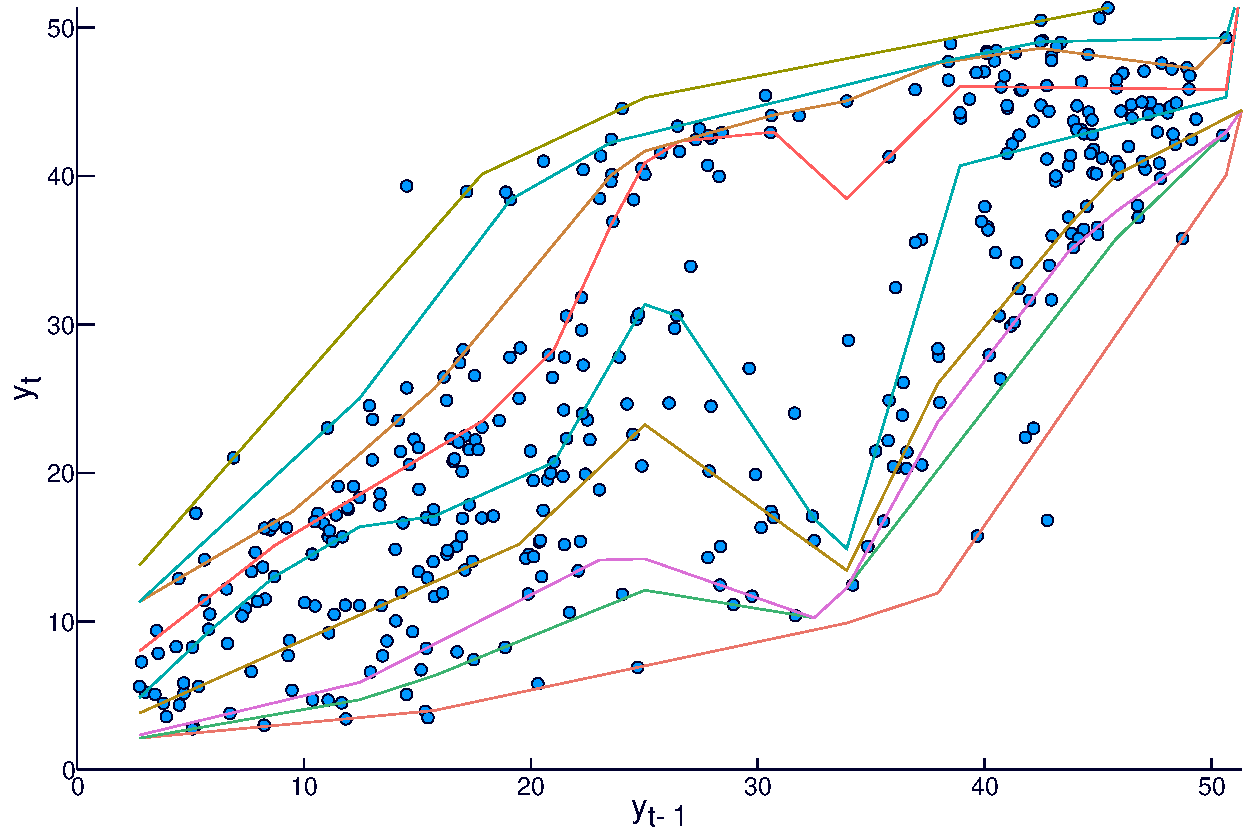
\includegraphics[width=\textwidth]{Figuras-DocRQ/icaraizinho-crossing-1}
      \subcaption{$\lambda_1 = 0, \, \lambda_2 = 1$}
     \end{minipage}
  \end{minipage}
  \begin{minipage}[t]{0.4\linewidth}
    \centering
    \begin{minipage}[t]{\linewidth}
      \centering     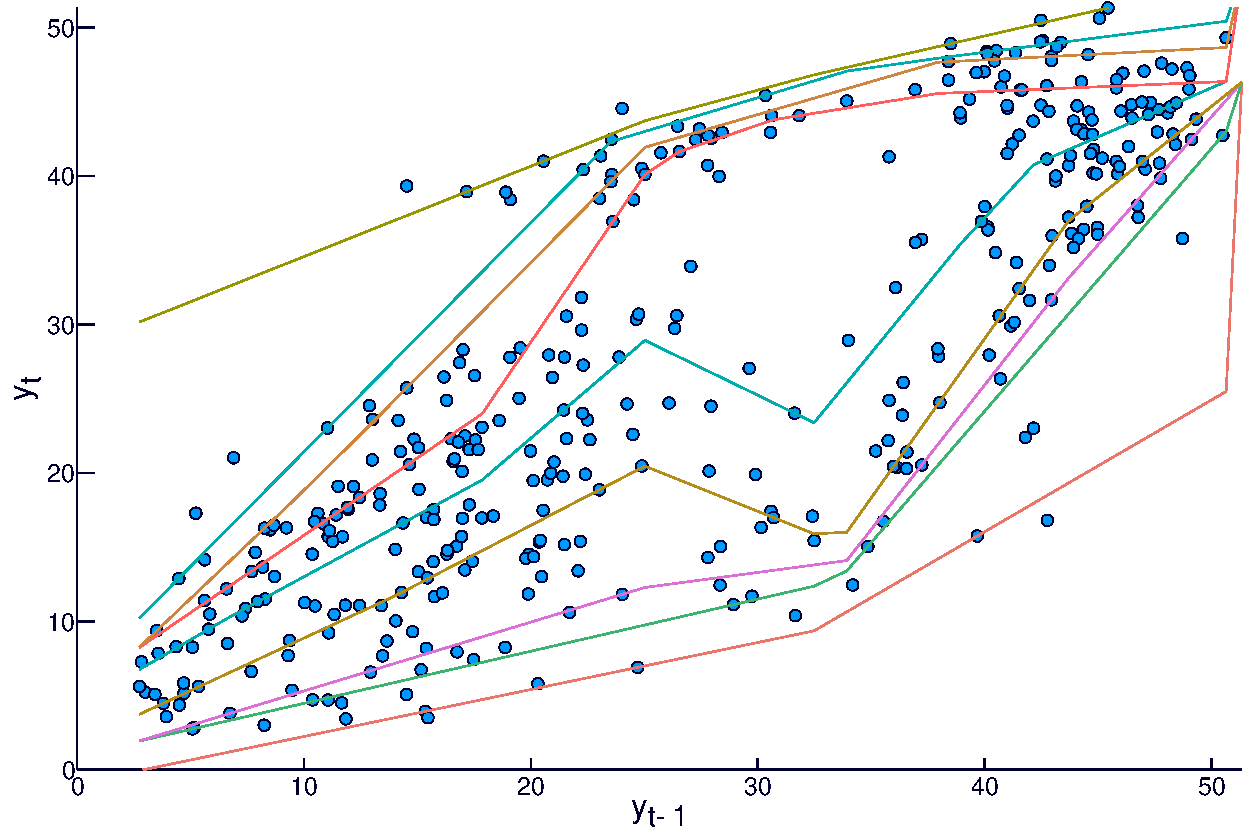
\includegraphics[width=\textwidth]{Figuras-DocRQ/icaraizinho-crossing-3}
      \subcaption{$\lambda_1 = 0, \, \lambda_2 = 3$}
    \end{minipage}
    \begin{minipage}[b]{\linewidth}
      \centering     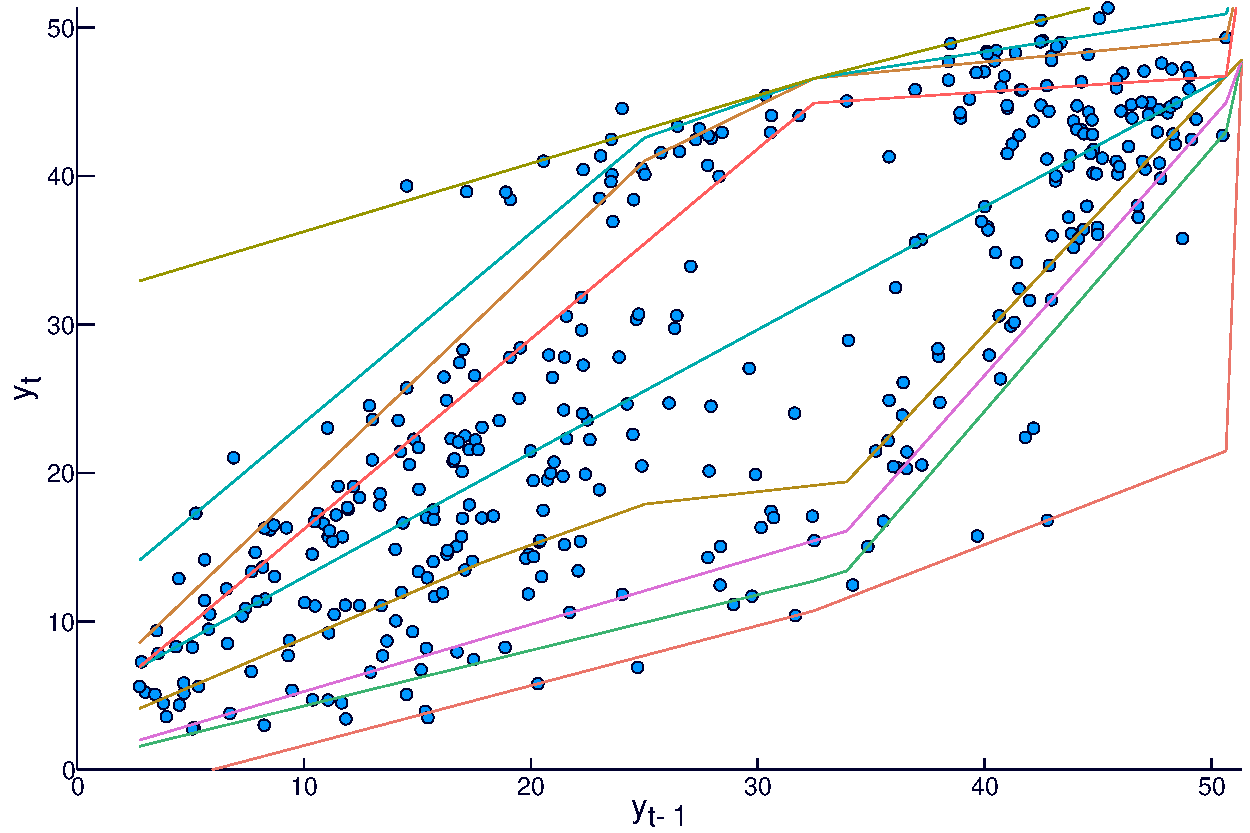
\includegraphics[width=\textwidth]{Figuras-DocRQ/icaraizinho-crossing-10}
      \subcaption{$\lambda_1 = 0, \, \lambda_2 = 10$}
    \end{minipage}
     \begin{minipage}[b]{\linewidth}
      \centering     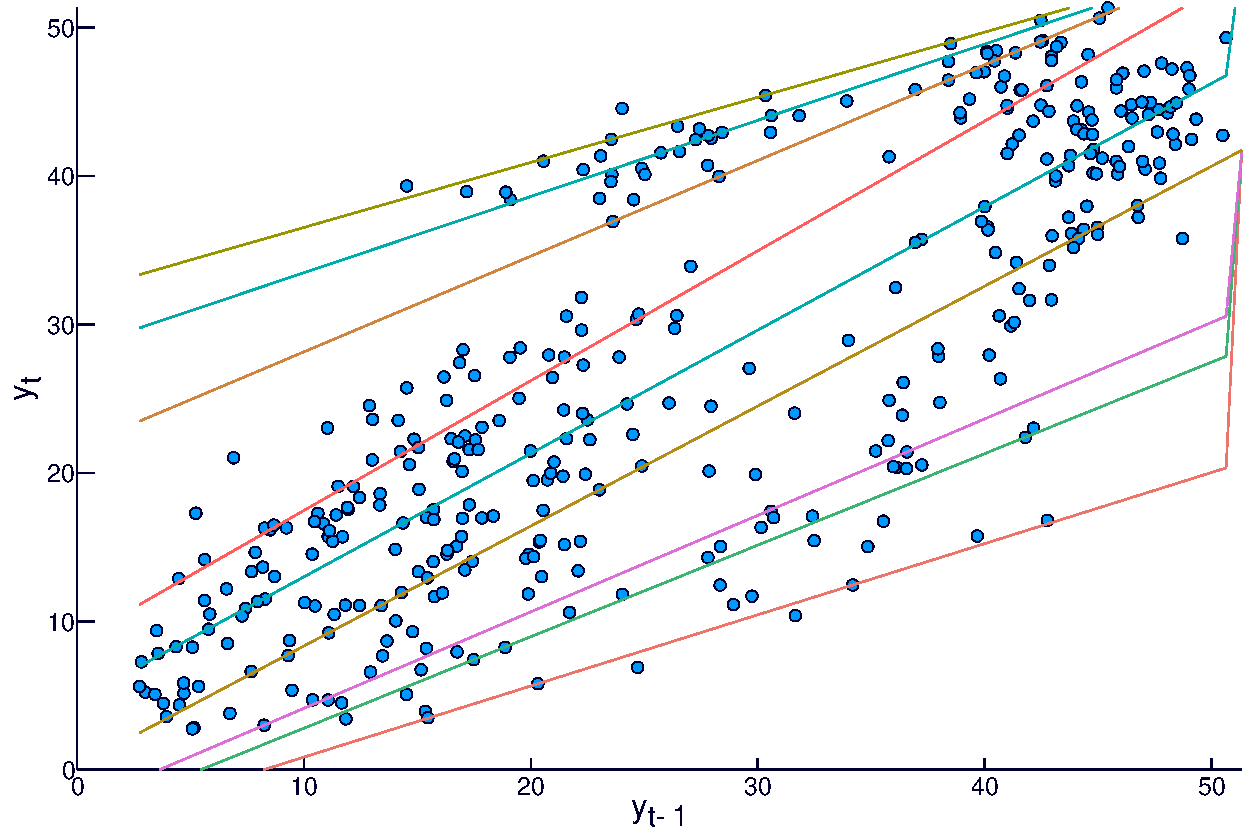
\includegraphics[width=\textwidth]{Figuras-DocRQ/icaraizinho-crossing-200}
      \subcaption{$\lambda_1 = 0, \, \lambda_2 = 200$}
      \label{fig:npqar-cross}
     \end{minipage}
  \end{minipage}
  \caption{Quantile estimations for a few different values of $\lambda_2$. The quantiles represented here are $\alpha = (5\%, 10\%, 25\%, 50\%, 75\%, 90\%, 95\%)$. When $\lambda_2 = 0.1$, on the upper left, we see a overfitting on the estimations. The other extreme case is also shown, when $\lambda_2=200$ the nonparametric estimator converges to the linear model.}
  \label{fig:npqar-results}
\end{figure*}

%The first issue is how to select an appropriate value for $\lambda_2$. A simple way is to do it by inspection, which means to test many different values and pick the one that suits best our needs by looking at them. The other alternative is to use a metric to which we can select the best tune. We can achieve this by using a cross-validation method, for example.

%The other issue occurs when we try to add more than one lag to the analysis at the same time. This happens because the problem solution is a set of points that we need to interpolate. This multivariate interpolation, however, is not easily solved, in the sense that we can either choose using a very naive estimator such as the K-nearest neighbors or just find another method that is not yet adopted for a wide range of applications.



